

% \chapter{\protect\hyperlink{chap:\thechapter}{Number Theory
% }
% \addtocontents{toc}{\protect\hypertarget{chap:\thechapter}{}}



\chap{Prime Numbers and Number Theory}


\section{Learning Goals}
\begin{tcolorbox}
 \textbf{\learninggoals}.
\tcblower
\begin{itemize}
\item Recognise   divisibility by  2,5,10 by inspection
\item Check for divisibility by 3,4,9 and 11 using mental or a pen-and-paper strategy
\item Check for divisibility by 7 using up to three iterations
\item Decompose  3-digit numbers to primes using the short division method
\item Decompose large numbers using calculator. \ie.  $\;123456789=3^2\times13717421$ 
\item Use prime
factorisation and short division to find the
greatest common divisor and the least
common multiple
\item Use the calculator method to find LCM and HCF for two  large numbers
\end{itemize}
\end{tcolorbox}


\section{Perform prime factorisation of positive integers}
Students are required to use prime
factorisation and short division to find the
greatest common divisor and the least
common multiple.
\section{GEogebra}
\section{{Number of prime factors}}
\begin{figure}[H]
\begin{center}
\hrefnoref{http://www.geogebra.org/m/E4Q3b4Bb}{\fbox{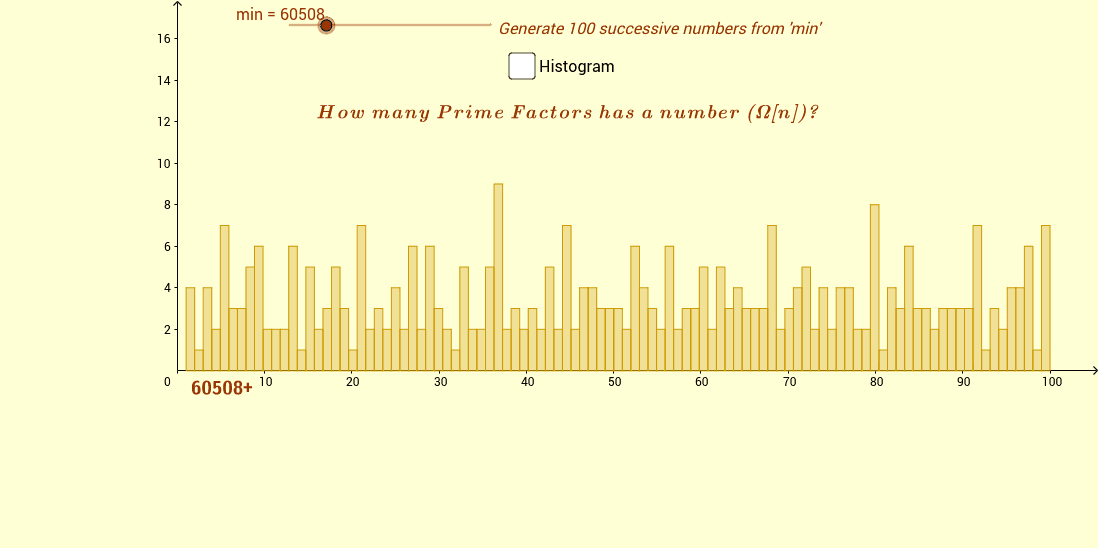
\includegraphics[width=120mm]{NUM/images/1}}}
\caption*{GeoGebra, \url{http://www.geogebra.org/m/E4Q3b4Bb}}
\end{center}
\end{figure}

\section{{sieve of eratosthenes}}
\begin{figure}[H]
\begin{center}
\hrefnoref{http://www.geogebra.org/m/FzeYCczw}{\fbox{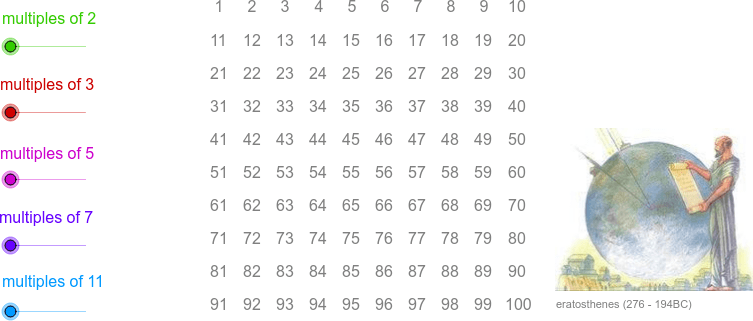
\includegraphics[width=120mm]{NUM/images/2}}}
\caption*{GeoGebra, \url{http://www.geogebra.org/m/FzeYCczw}}
\end{center}
\end{figure}

\section{{Prime Factors - step by step}}
Enter a positive integer and explore it's decomposition into prime factors.

If the factoring doesn't fit in the screen height - a scroll bar appears on the left.

\begin{figure}[H]
\begin{center}
\hrefnoref{http://www.geogebra.org/m/xZajPpB3}{\fbox{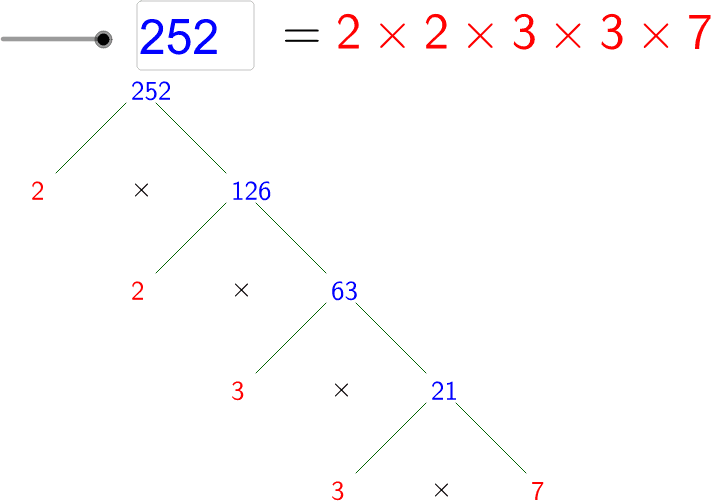
\includegraphics[width=120mm]{NUM/images/3}}}
\caption*{GeoGebra, \url{http://www.geogebra.org/m/xZajPpB3}}
\end{center}
\end{figure}

\section{{Prime Factors 2 to 150}}
\begin{figure}[H]
\begin{center}
\hrefnoref{http://www.geogebra.org/m/bN4gadJw}{\fbox{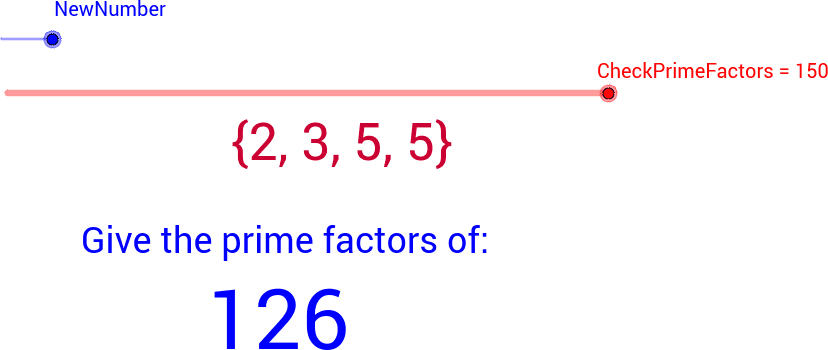
\includegraphics[width=120mm]{NUM/images/4}}}
\caption*{GeoGebra, \url{http://www.geogebra.org/m/bN4gadJw}}
\end{center}
\end{figure}

\section{{Factorization - Visual illustration of divisor pairs}}
\begin{enumerate}[label=\arabic*.]

\item Enter different integers (whole numbers).

\item See what prime numbers compose your integer.

\item Press the prime factors buttons and see how your number can be produced by multiplying different pairs of numbers.

\item How many different pairs that produce your number are there?

\end{enumerate}

\begin{figure}[H]
\begin{center}
\hrefnoref{http://www.geogebra.org/m/GJ3khRQj}{\fbox{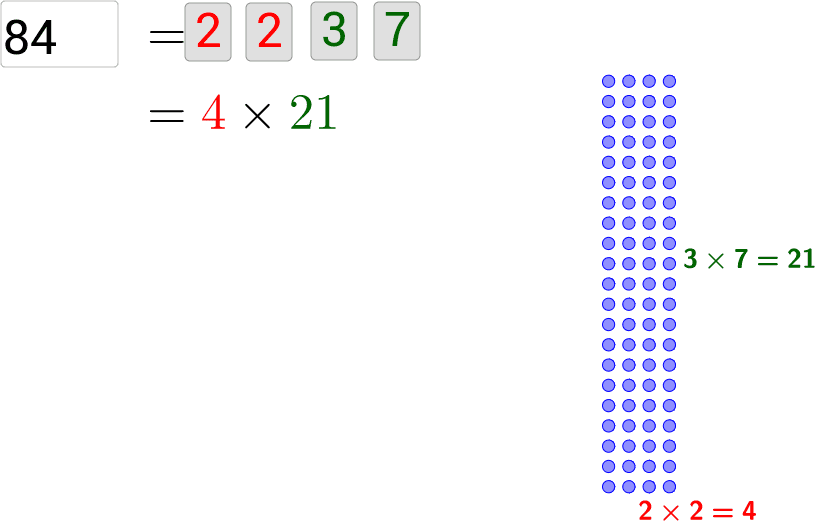
\includegraphics[width=120mm]{NUM/images/5}}}
\caption*{GeoGebra, \url{http://www.geogebra.org/m/GJ3khRQj}}
\end{center}
\end{figure}

\section{{Fundamental Theorem of Arithmetic}}
\begin{figure}[H]
\begin{center}
\hrefnoref{http://www.geogebra.org/m/XrdVXnUf}{\fbox{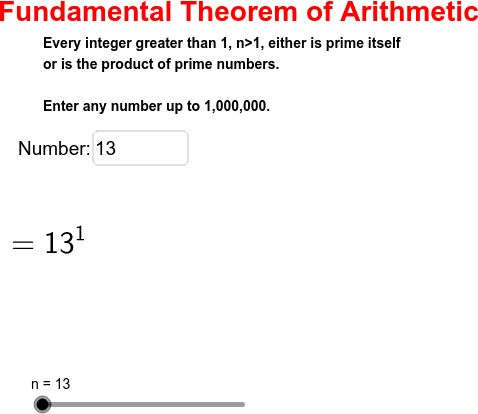
\includegraphics[width=95.6mm]{NUM/images/6}}}
\caption*{GeoGebra, \url{http://www.geogebra.org/m/XrdVXnUf}}
\end{center}
\end{figure}

\section{{Smallest k such that m ×  k  is a perfect cube}}
\begin{figure}[H]
\begin{center}
\hrefnoref{http://www.geogebra.org/m/a3ksuvbh}{\fbox{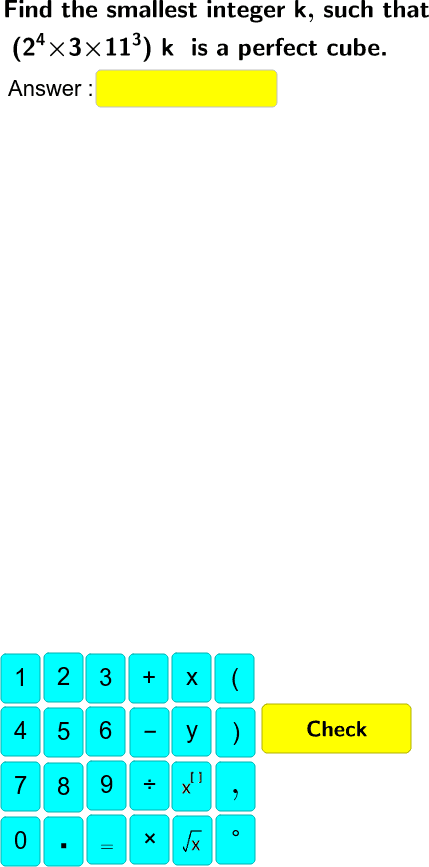
\includegraphics[width=85.8mm]{NUM/images/7}}}
\caption*{GeoGebra, \url{http://www.geogebra.org/m/a3ksuvbh}}
\end{center}
\end{figure}

\section{{Prime Factorisation of Positive Integers }}
\begin{figure}[H]
\begin{center}
\hrefnoref{http://www.geogebra.org/m/hn7zs5dh}{\fbox{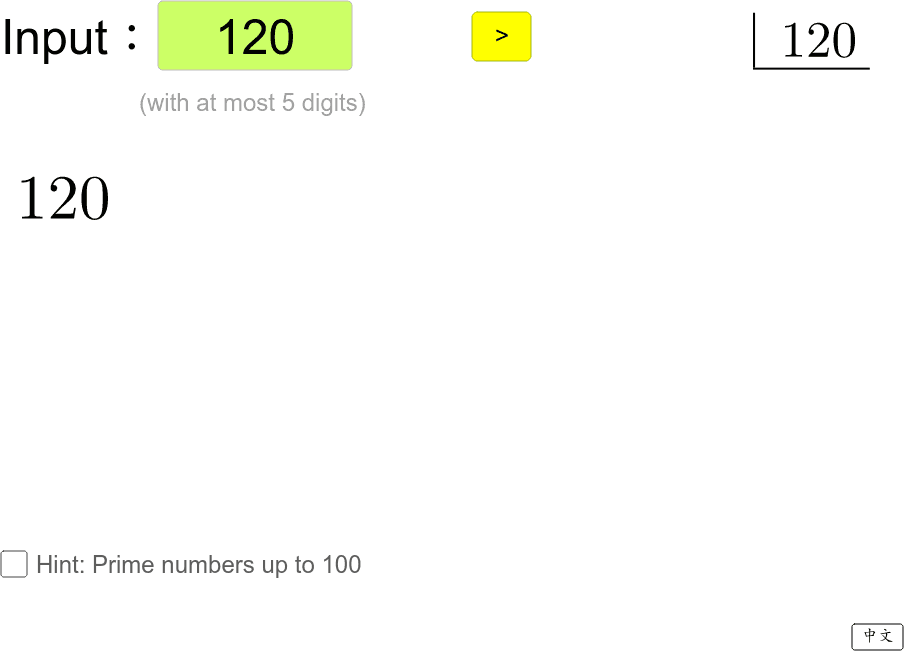
\includegraphics[width=120mm]{NUM/images/8}}}
\caption*{GeoGebra, \url{http://www.geogebra.org/m/hn7zs5dh}}
\end{center}
\end{figure}

\section{{Writing a number as a product of its prime factors}}
\begin{figure}[H]
\begin{center}
\hrefnoref{http://www.geogebra.org/m/zkbbyggw}{\fbox{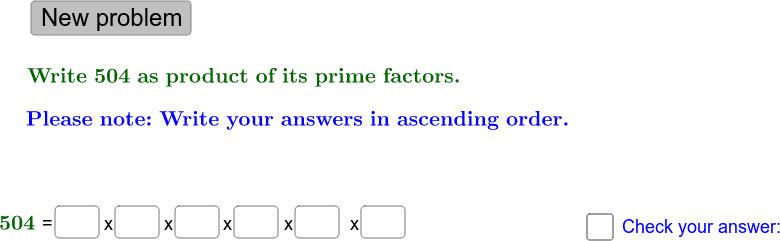
\includegraphics[width=120mm]{NUM/images/9}}}
\caption*{GeoGebra, \url{http://www.geogebra.org/m/zkbbyggw}}
\end{center}
\end{figure}

\section{{Prime Factors}}
Guess the prime factors of the blue number.  Use the red slider to check your answer.  Slide NewNumber to generate a new number between 2 and 256.

\begin{figure}[H]
\begin{center}
\hrefnoref{http://www.geogebra.org/m/k4suprEZ}{\fbox{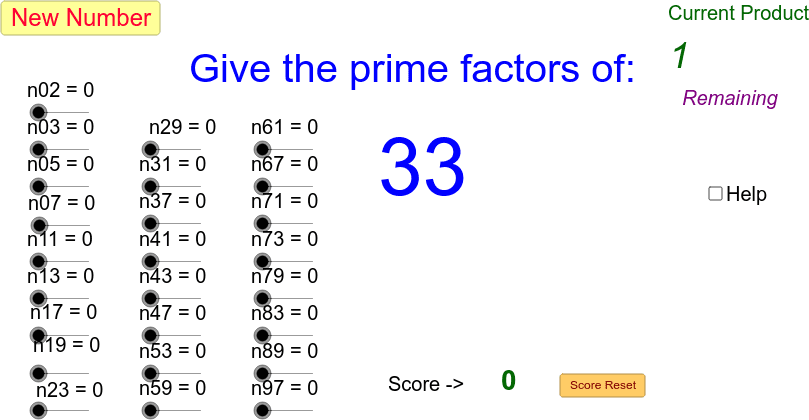
\includegraphics[width=120mm]{NUM/images/10}}}
\caption*{GeoGebra, \url{http://www.geogebra.org/m/k4suprEZ}}
\end{center}
\end{figure}

Play with a friend.

Revised:  \href {http://tube.geogebra.org/m/22178}{Terry Lee Lindenmuth — November 16, 2012 - 2:40 PM} \textnormal{\cite{{1}}}

Primes not available: 101, 103, 107, 109, 113, 127, 131, 137, 139, 149, 151, 157, 163, 167, 173, 179, 181, 191, 193, 197, 199, 211, 223, 227, 229, 233, 241, 251

\section{{Sieve of Eratosthenes}}
\begin{figure}[H]
\begin{center}
\hrefnoref{http://www.geogebra.org/m/ZWDkYU4t}{\fbox{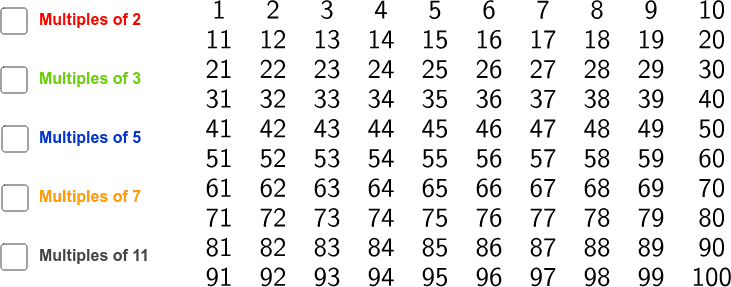
\includegraphics[width=120mm]{NUM/images/11}}}
\caption*{GeoGebra, \url{http://www.geogebra.org/m/ZWDkYU4t}}
\end{center}
\end{figure}

\section{{Prime before and after}}
Test your knowledge about Prime numbers.

Think the numbers and check.

Are you right.

Great!!!!

\begin{figure}[H]
\begin{center}
\hrefnoref{http://www.geogebra.org/m/S7yX9fbe}{\fbox{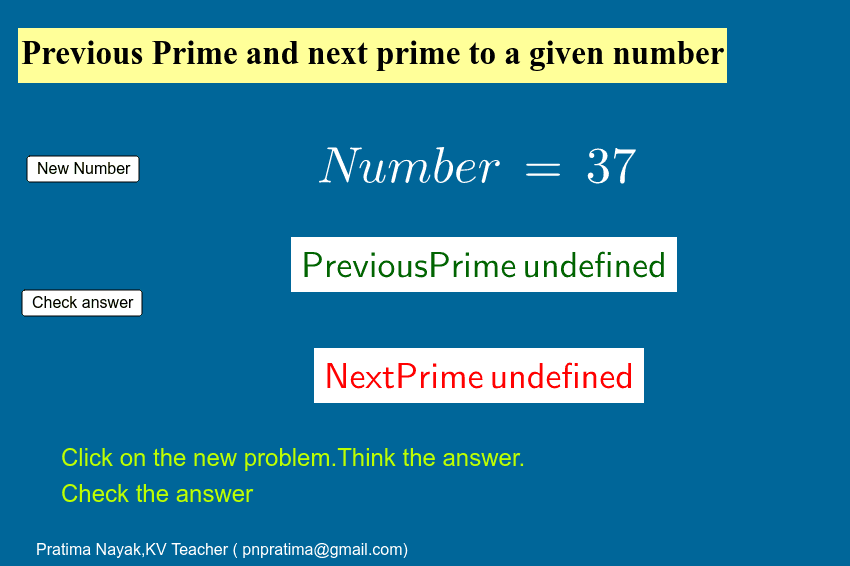
\includegraphics[width=120mm]{NUM/images/12}}}
\caption*{GeoGebra, \url{http://www.geogebra.org/m/S7yX9fbe}}
\end{center}
\end{figure}









\section{Perform prime factorisation of positive integers}
Students are required to use prime
factorisation and short division to find the
greatest common divisor and the least
common multiple.
\section{GEogebra}
\section{{Number of prime factors}}
\begin{figure}[H]
\begin{center}
\hrefnoref{http://www.geogebra.org/m/E4Q3b4Bb}{\fbox{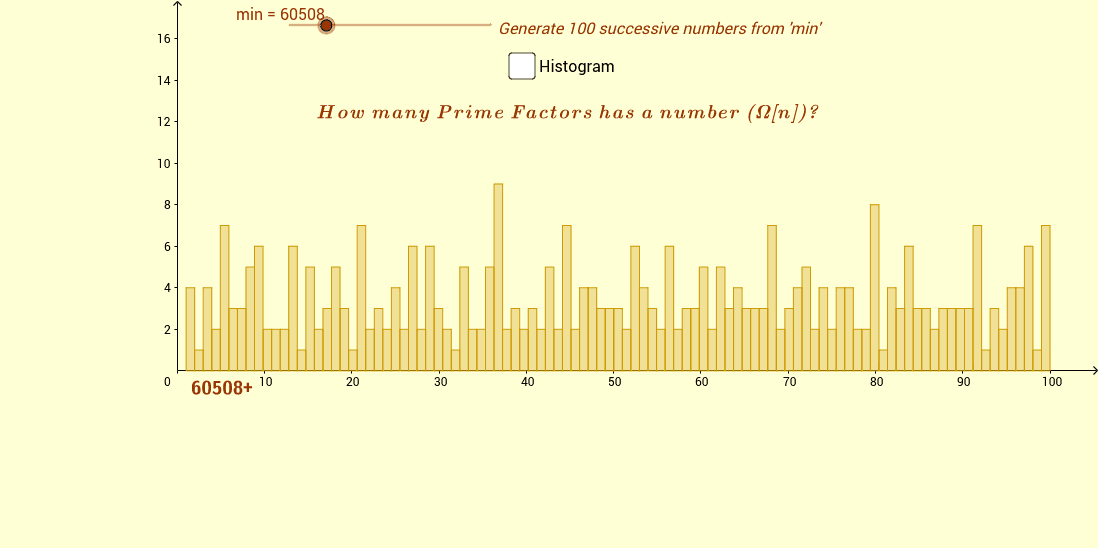
\includegraphics[width=120mm]{NUM/images/1}}}
\caption*{GeoGebra, \url{http://www.geogebra.org/m/E4Q3b4Bb}}
\end{center}
\end{figure}

\section{{sieve of eratosthenes}}
\begin{figure}[H]
\begin{center}
\hrefnoref{http://www.geogebra.org/m/FzeYCczw}{\fbox{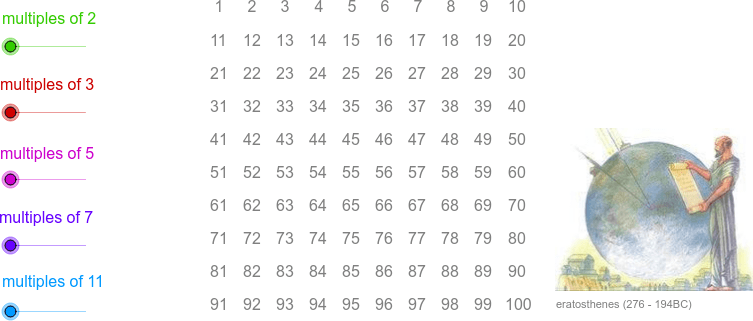
\includegraphics[width=120mm]{NUM/images/2}}}
\caption*{GeoGebra, \url{http://www.geogebra.org/m/FzeYCczw}}
\end{center}
\end{figure}

\section{{Prime Factors - step by step}}
Enter a positive integer and explore it's decomposition into prime factors.

If the factoring doesn't fit in the screen height - a scroll bar appears on the left.

\begin{figure}[H]
\begin{center}
\hrefnoref{http://www.geogebra.org/m/xZajPpB3}{\fbox{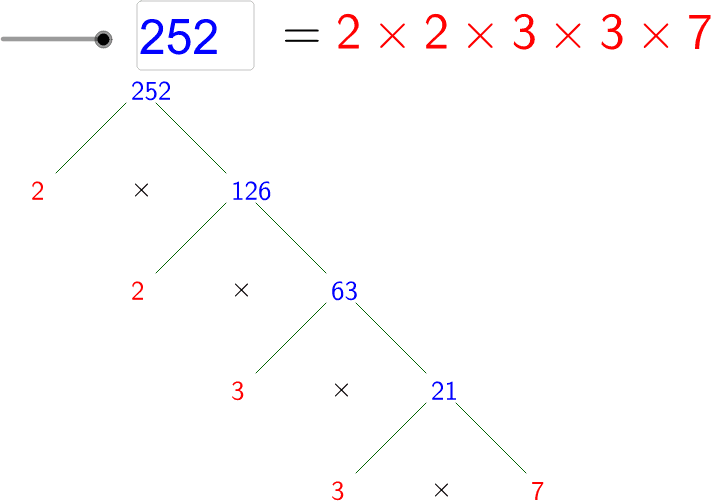
\includegraphics[width=120mm]{NUM/images/3}}}
\caption*{GeoGebra, \url{http://www.geogebra.org/m/xZajPpB3}}
\end{center}
\end{figure}

\section{{Prime Factors 2 to 150}}
\begin{figure}[H]
\begin{center}
\hrefnoref{http://www.geogebra.org/m/bN4gadJw}{\fbox{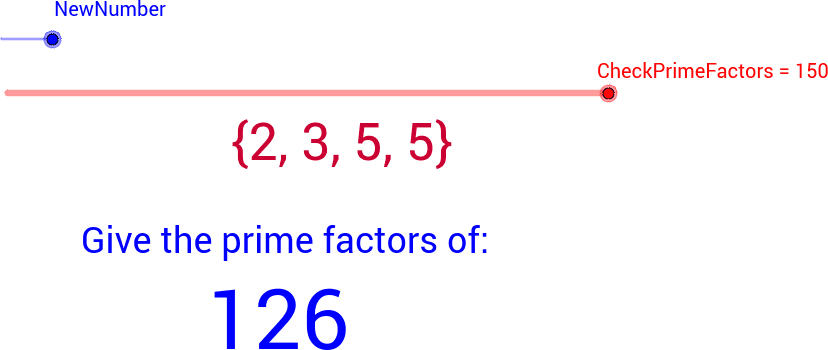
\includegraphics[width=120mm]{NUM/images/4}}}
\caption*{GeoGebra, \url{http://www.geogebra.org/m/bN4gadJw}}
\end{center}
\end{figure}

\section{{Factorization - Visual illustration of divisor pairs}}
\begin{enumerate}[label=\arabic*.]

\item Enter different integers (whole numbers).

\item See what prime numbers compose your integer.

\item Press the prime factors buttons and see how your number can be produced by multiplying different pairs of numbers.

\item How many different pairs that produce your number are there?

\end{enumerate}

\begin{figure}[H]
\begin{center}
\hrefnoref{http://www.geogebra.org/m/GJ3khRQj}{\fbox{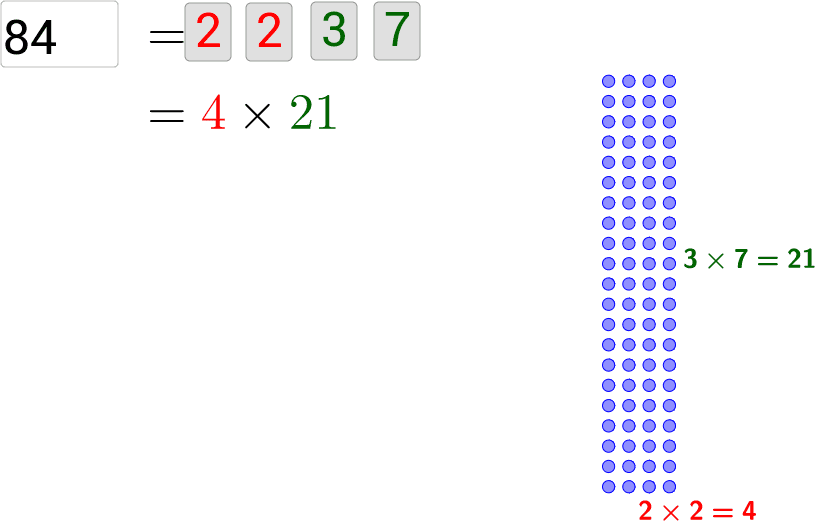
\includegraphics[width=120mm]{NUM/images/5}}}
\caption*{GeoGebra, \url{http://www.geogebra.org/m/GJ3khRQj}}
\end{center}
\end{figure}

\section{{Fundamental Theorem of Arithmetic}}
\begin{figure}[H]
\begin{center}
\hrefnoref{http://www.geogebra.org/m/XrdVXnUf}{\fbox{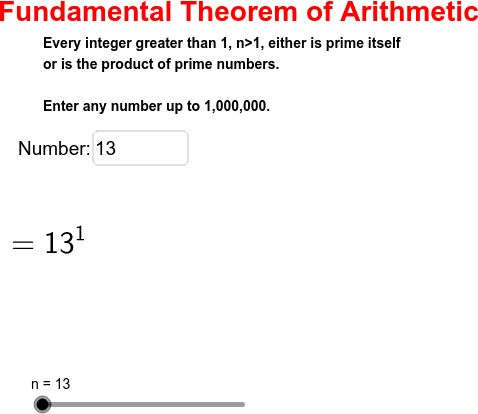
\includegraphics[width=95.6mm]{NUM/images/6}}}
\caption*{GeoGebra, \url{http://www.geogebra.org/m/XrdVXnUf}}
\end{center}
\end{figure}

\section{{Smallest k such that m ×  k  is a perfect cube}}
\begin{figure}[H]
\begin{center}
\hrefnoref{http://www.geogebra.org/m/a3ksuvbh}{\fbox{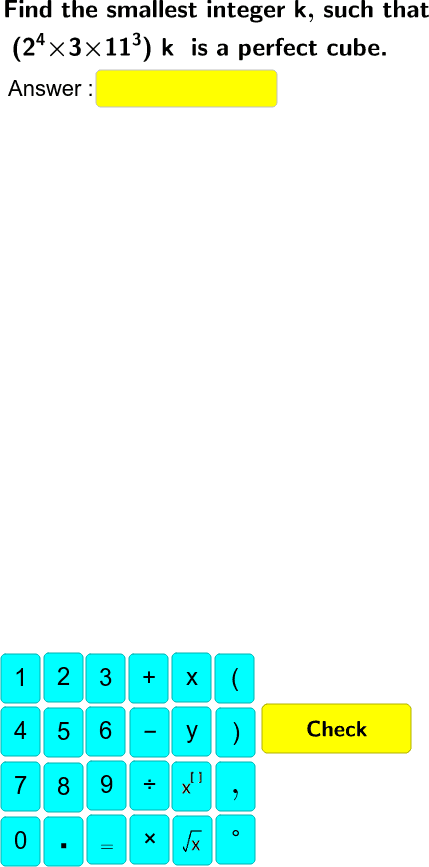
\includegraphics[width=85.8mm]{NUM/images/7}}}
\caption*{GeoGebra, \url{http://www.geogebra.org/m/a3ksuvbh}}
\end{center}
\end{figure}

\section{{Prime Factorisation of Positive Integers }}
\begin{figure}[H]
\begin{center}
\hrefnoref{http://www.geogebra.org/m/hn7zs5dh}{\fbox{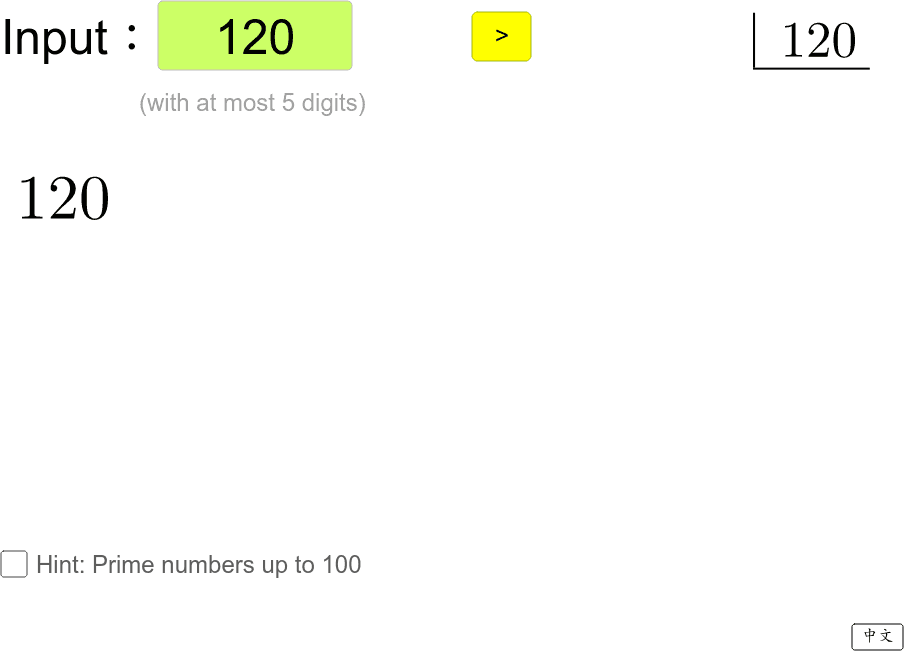
\includegraphics[width=120mm]{NUM/images/8}}}
\caption*{GeoGebra, \url{http://www.geogebra.org/m/hn7zs5dh}}
\end{center}
\end{figure}

\section{{Writing a number as a product of its prime factors}}
\begin{figure}[H]
\begin{center}
\hrefnoref{http://www.geogebra.org/m/zkbbyggw}{\fbox{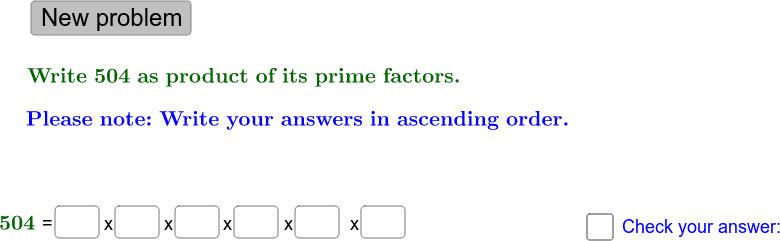
\includegraphics[width=120mm]{NUM/images/9}}}
\caption*{GeoGebra, \url{http://www.geogebra.org/m/zkbbyggw}}
\end{center}
\end{figure}

\section{{Prime Factors}}
Guess the prime factors of the blue number.  Use the red slider to check your answer.  Slide NewNumber to generate a new number between 2 and 256.

\begin{figure}[H]
\begin{center}
\hrefnoref{http://www.geogebra.org/m/k4suprEZ}{\fbox{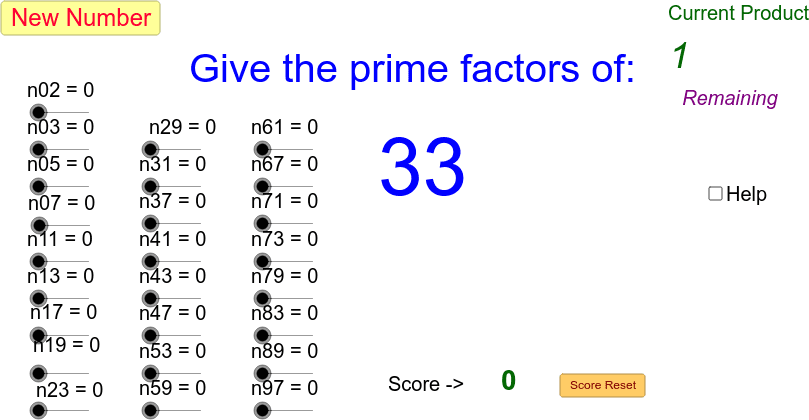
\includegraphics[width=120mm]{NUM/images/10}}}
\caption*{GeoGebra, \url{http://www.geogebra.org/m/k4suprEZ}}
\end{center}
\end{figure}

Play with a friend.

Revised:  \href {http://tube.geogebra.org/m/22178}{Terry Lee Lindenmuth — November 16, 2012 - 2:40 PM} \textnormal{\cite{{1}}}

Primes not available: 101, 103, 107, 109, 113, 127, 131, 137, 139, 149, 151, 157, 163, 167, 173, 179, 181, 191, 193, 197, 199, 211, 223, 227, 229, 233, 241, 251

\section{{Sieve of Eratosthenes}}
\begin{figure}[H]
\begin{center}
\hrefnoref{http://www.geogebra.org/m/ZWDkYU4t}{\fbox{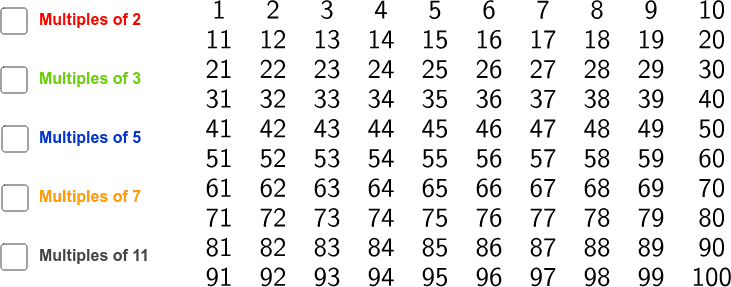
\includegraphics[width=120mm]{NUM/images/11}}}
\caption*{GeoGebra, \url{http://www.geogebra.org/m/ZWDkYU4t}}
\end{center}
\end{figure}

\section{{Prime before and after}}
Test your knowledge about Prime numbers.

Think the numbers and check.

Are you right.

Great!!!!

\begin{figure}[H]
\begin{center}
\hrefnoref{http://www.geogebra.org/m/S7yX9fbe}{\fbox{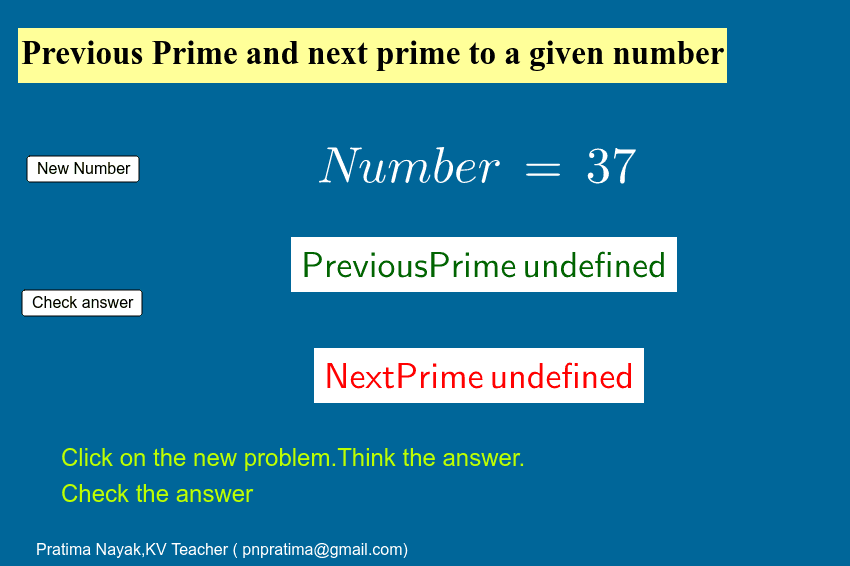
\includegraphics[width=120mm]{NUM/images/12}}}
\caption*{GeoGebra, \url{http://www.geogebra.org/m/S7yX9fbe}}
\end{center}
\end{figure}

\section{Multiples}
We know that $12$ equals $3$ times $4$. In other words, $12$ equals some integer times $4$. For that reason, we say that $12$ is a \textbf{multiple}  of 4.
\begin{definition}
Let $\color[rgb]{0.11,0.21,0.37}a$ and $\color[rgb]{0.11,0.21,0.37}b$ be numbers. We say that $\color[rgb]{0.11,0.21,0.37}a$ is a multiple of $\color[rgb]{0.11,0.21,0.37}b$ if $\color[rgb]{0.11,0.21,0.37}a$ equals $\color[rgb]{0.11,0.21,0.37}b$ times some integer. In other words, $\color[rgb]{0.11,0.21,0.37}a$ is a multiple of $\color[rgb]{0.11,0.21,0.37}b$ if there is an integer $\color[rgb]{0.11,0.21,0.37}n$ such that $\color[rgb]{0.11,0.21,0.37}a = bn$.
\end{definition}
For instance, 7 is not a multiple of 4, because we cannot write 7 as the  \textbf{product}  of 4 and an integer. Note that $-12$ is a multiple of $4$, because $-12$ equals $-3$ times $4$. Similarly, $0$ is a multiple of $4$, because $0$ equals $0$ times $4$.

In this chapter, we’ll talk about division differently than we did in Chapter 1. We’ll use the “quotient and remainder” concept of division, which you probably used when you first learned about division. As an example, when we divide 13 by 4, the quotient is 3 and the remainder is 1.

Using this view of division, we can say that an integer $a$ is a multiple of an integer $b$ if $a$ divided by $b$ has remainder 0. So, for example, 12 is a multiple of 4 because $12$ divided by $4$ has remainder 0, while 13 is not a multiple of 4 because $13$ divided by $4$ has remainder 1.
\section{find the greatest common divisor and the least
common multiple}

At Key Stage 2, students are required to find
the greatest common divisor and the least
common multiple of two numbers by listing
their multiples and factors, and using short
division.

\section{find the greatest common divisor and the least
common multiple}

At Key Stage 2, students are required to find
the greatest common divisor and the least
common multiple of two numbers by listing
their multiples and factors, and using short
division.



The terms “H.C.F.”, “gcd”, etc. can be used.







\section{}








\section{}

















\section{}













